% =====================================================================
%  Chapter 5 — Evaluation and Results  (~3,000 words) — THE MARKS
%  DRAFT generated 2026-07-18.
%  Numbers: macros come from results/tables/numbers.tex (log-generated).
%  Literals in this chapter fall into two classes, both annotated:
%    [ANALYSIS] — produced by a named analysis script over the raw logs
%                 (gate ablation, distraction study, chunk relevance,
%                 attribution). Re-run the script to verify.
%    [FROZEN]   — deliberately retained pilot/uncalibrated historical values
%                 kept for contrast; do NOT "update" them.
% =====================================================================
\chapter{Evaluation and Results}
\label{ch:eval}

\section{Experimental Setup}
\label{sec:eval-setup}

All experiments run Llama-3.2-3B-Instruct, 4-bit quantised (Q4\_K\_M),
served by \texttt{llama.cpp} on CPU only (medium hardware tier), with greedy
decoding and fixed seed --- every run is deterministic and was verified to
replay exactly (Section~\ref{sec:eval-ablation}). Two question sets of
$n=\nQuestions{}$ each are used: MIRAGE MMLU-Med multiple-choice questions,
scored by exact letter match, and PubMedQA (\texttt{pqa\_labeled}) open-ended
questions, scored by mean token-level $F_1$ against the gold paragraph.
Binary correctness is not reported for open-ended answers because
thresholding $F_1$ at zero yields $\sim$98\% and measures nothing. The
retrieval corpus is the 425,847-chunk medical corpus of
Section~\ref{sec:impl-corpus}. Secondary metrics are retrieval rate, mean
per-query latency, and estimated energy.

The sample size must be conceded at the outset: $n=\nQuestions{}$ per
condition is small, and its cost is visible in the confidence intervals of
Section~\ref{sec:eval-main}. Where a result is a \emph{count} over the
sample (retrieval rate) it is exact for that sample; where it is an
\emph{estimate} of a population difference (accuracy gaps) the interval is
reported and taken seriously.

\section{Main Comparison}
\label{sec:eval-main}

% AUTO-GENERATED by scripts/generate_tables.py -- DO NOT EDIT.
% Regenerate with: python scripts/generate_tables.py
% Every number is computed from results/raw_logs/ via evaluation.loading.
% git c8f491b | 2026-08-04 21:39
\begin{table}[t]
  \centering
  \begin{tabular}{llccc}
    \toprule
    Policy & Type & Accuracy / F1 & Retrieval & Latency/q \\
    \midrule
    P1 always-retrieve & MCQ & 45.5\% & 100.0\% & 27\,s \\
    P4 hybrid & MCQ & 45.5\% & 100.0\% & 25\,s \\
    P3 closed-book$^\dagger$ & MCQ & 62.0\% & 0.0\% & 57\,s \\
    P5 gated (calib.) & MCQ & 54.5\% & 49.5\% & 153\,s \\
    \midrule
    P1 always-retrieve & open & 0.220 & 100.0\% & 23\,s \\
    P3 closed-book$^\dagger$ & open & 0.190 & 0.0\% & 27\,s \\
    P5 gated (calib.) & open & 0.211 & 79.0\% & 380\,s \\
    \bottomrule
  \end{tabular}
  \caption{All policies on the real MedCorp corpus (425{,}847 chunks), quantised
  Llama-3.2-3B. Multiple-choice is scored by accuracy; open-ended by mean token-F1
  (binary accuracy is not defined for open-ended answers -- see
  Section~\ref{sec:impl-harness}). $^{\dagger}$P3 never retrieves, so its result is
  corpus-independent; it is a paired run over the identical question set.}
  \label{tab:main-results}
\end{table}


\begin{figure}[t]
  \centering
  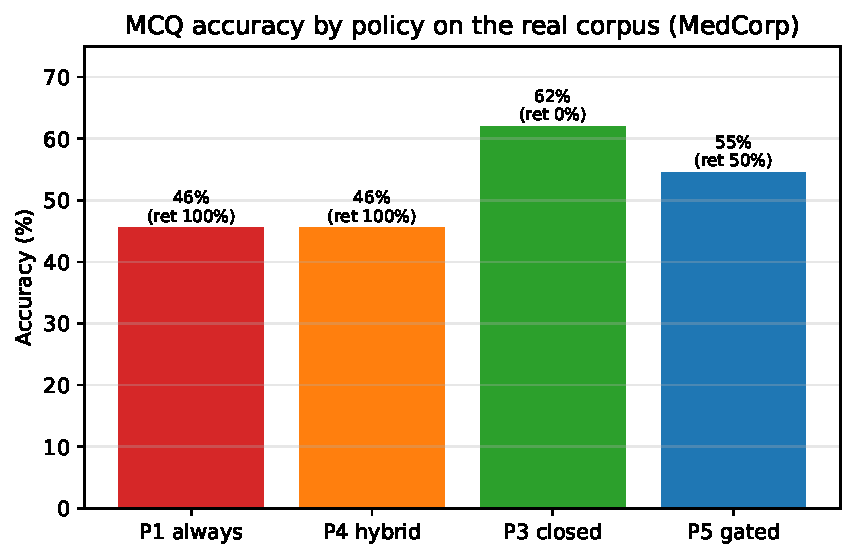
\includegraphics[width=0.75\linewidth]{results/figures/fig_medcorp_policies}
  \caption{MCQ accuracy by policy on the real corpus. Among retrieving
    policies, gated P5 (\accPfiveMcq{}, retrieving \retPfiveMcq{} of the
    time) beats always-retrieve P1/P4 (\accPoneMcq{}, \retPoneMcq{});
    closed-book P3 (\accPthreeMcq{}) remains highest.}
  \label{fig:medcorp-policies}
\end{figure}

Three claims follow from Table~\ref{tab:main-results}, in decreasing order of
certainty.

\paragraph{1. Selective retrieval beats always-retrieve --- cost exactly,
accuracy suggestively.} Among the retrieving policies, gated P5 reaches
\accPfiveMcq{} against \accPoneMcq{} for both P1 (always-retrieve) and P4
(hybrid), while retrieving on only \retPfiveMcq{} of queries. The two halves
of this claim carry different evidential weight and are stated separately.
The retrieval-cost halving is a \emph{count}, not an estimate: P5 answered
half the queries without touching the corpus at all. The accuracy gain of
\diffPfivePone{}pp, however, carries a 95\% confidence interval of
\diffPfivePoneCI{} at $n=\nQuestions{}$ --- an interval that includes zero.
The gain is therefore \emph{consistent with} a genuine improvement rather
than proof of one; this evaluation is not powered to establish it. Stating
that plainly costs the headline little and buys the analysis its
credibility.

\paragraph{2. Closed-book still leads on multiple choice.} P3
(\accPthreeMcq{}) tops every retrieving policy on MCQ. MIRAGE's
multiple-choice questions predominantly probe textbook knowledge the 3B
model already holds parametrically; Sections~\ref{sec:eval-distraction}
and~\ref{sec:eval-protective} dissect \emph{why} retrieval fails to help
here, and the answer is more interesting than ``the model is weak.''

\paragraph{3. Open-ended inverts the ordering.} On PubMedQA, P5
($F_1 = \f1PfiveOpen{}$) edges above closed-book P3 (\f1PthreeOpen{}), with
P1 at \f1PoneOpen{}. Where the model \emph{lacks} the specific study
findings, retrieval genuinely adds information. The MCQ/open-ended split is
not an inconsistency to be explained away --- it is the finding: retrieval
helps precisely when the model does not already know, which is exactly the
condition a gate exists to detect.

\section{Why the Defaults Never Fired: Calibration Non-Transfer}
\label{sec:eval-calibration}

\begin{figure}[t]
  \centering
  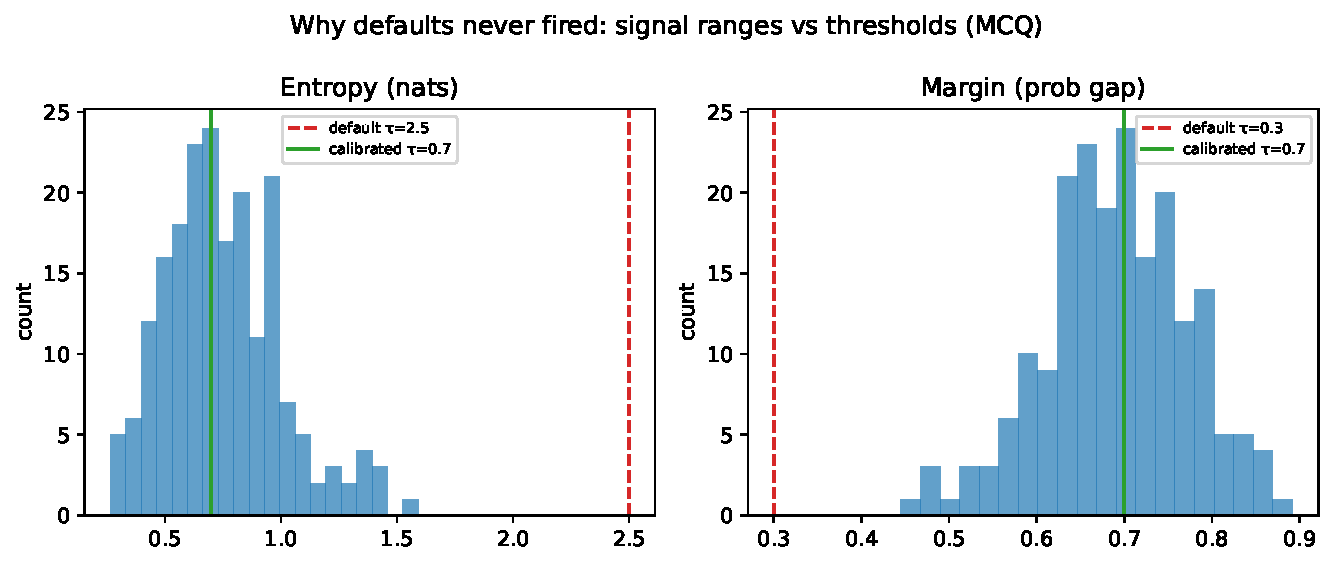
\includegraphics[width=\linewidth]{results/figures/fig_signals}
  \caption{Gate-signal distributions on \nQuestions{} MCQs versus thresholds.
    The literature defaults (red) lie entirely outside the observed signal
    range; the calibrated thresholds (green, $\tau=0.70$) sit within the
    signal mass.}
  \label{fig:signals}
\end{figure}

At the thresholds inherited from the general-domain literature
($\tau_H = 2.5$ nats, $\tau_M = 0.3$), the gate retrieved on \emph{zero} of
\nQuestions{} questions, and P5 collapsed onto closed-book P3 exactly.
Figure~\ref{fig:signals} shows why: on the 4-bit quantised model, greedy
draft distributions are sharply peaked, so observed mean entropy spans only
0.27--1.59 nats % [FROZEN] uncalibrated-run signal range, week2 logs
--- never approaching the 2.5-nat trigger --- and the top-two margin spans
0.45--0.89, never falling below the 0.3 trigger. Neither threshold is
\emph{physically reachable}. Only the threshold-free hallucination probe
ever voted to retrieve (80 of 200 questions), and under a 2-of-3 majority a
lone vote cannot carry the decision.

This is an empirical finding, not an implementation fault: \textbf{gate
thresholds calibrated on full-precision general-domain models do not
transfer to a small quantised model.} Quantisation sharpens output
distributions, relocating the entire signal range.

Recalibration is cheap because it is \emph{offline}. Every run logs the raw
per-gate signal per query, so the retrieve/skip decision can be replayed at
any threshold without invoking the model --- a sweep over a threshold grid
takes seconds rather than the hours a live re-run would cost. A single
global operating point $\tau_H = \tau_M = 0.70$ places retrieval at
\retPfiveMcq{} on MCQ and \retPfiveOpen{} on open-ended questions. The
higher open-ended rate is itself informative: the probe's draft-agreement
signal disagrees far more often on free text than on a choice among four
letters, so the ensemble crosses its voting threshold more readily.

\section{The Corpus Was the Bottleneck}
\label{sec:eval-corpus}

\begin{figure}[t]
  \centering
  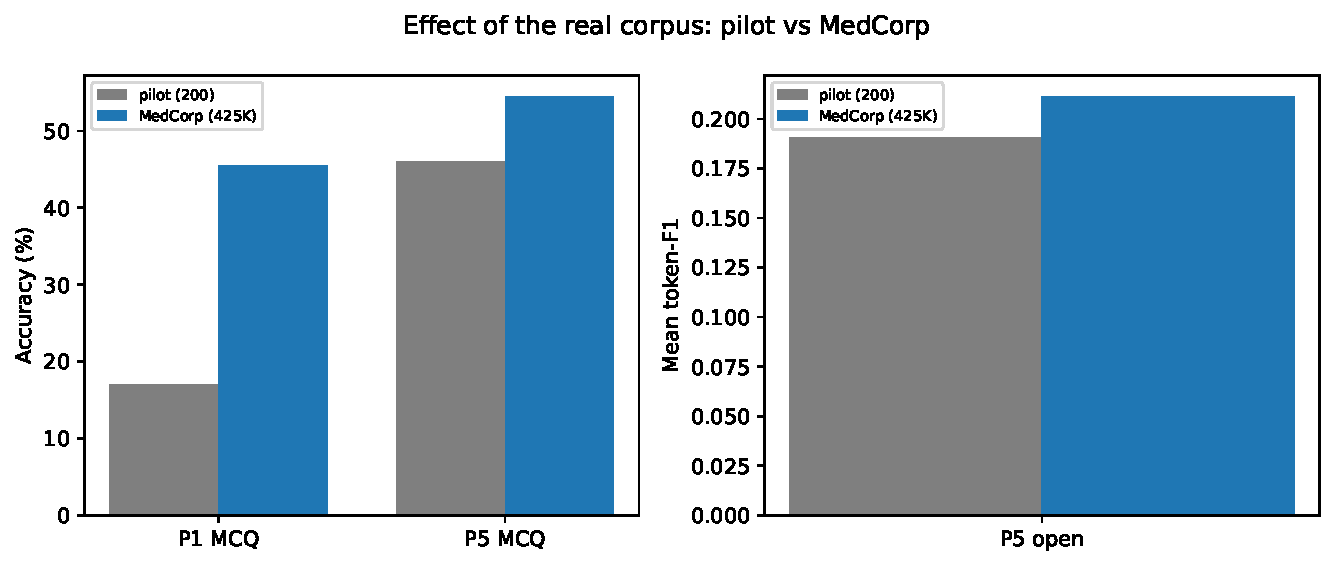
\includegraphics[width=\linewidth]{results/figures/fig_corpus_effect}
  \caption{Effect of replacing the 200-chunk pilot corpus with the
    426K-chunk medical corpus: every retrieving policy improves sharply.}
  \label{fig:corpus-effect}
\end{figure}

On the 200-chunk pilot corpus, always-retrieve P1 scored 17\%
% [FROZEN] pilot-corpus result, retained for contrast
and \emph{calibrated} P5 dropped from \accPthreeMcq{} (when its gate never
fired) to 45.5\% (once it began retrieving at 50\%).
% [FROZEN] pilot calibrated-P5 result
The gate was functioning exactly as designed --- firing at the calibrated
rate --- yet firing made the policy worse, because the corpus contained
almost nothing worth retrieving. The general principle, and the cleanest
lesson in this dissertation: \textbf{gated retrieval inherits the quality of
the corpus it retrieves from.} A gate cannot rescue retrieval from an empty
well; on a poor corpus the safest gate is one that retrieves less.

Replacing the pilot with the real corpus lifted P1 from 17\% to
\accPoneMcq{} (Figure~\ref{fig:corpus-effect}), retrospectively confirming
the diagnosis: the earlier collapse was a property of the corpus, not of the
gating machinery.

\section{Retrieval as Distraction}
\label{sec:eval-distraction}
% [ANALYSIS] paired P1-vs-P3 study over p1_medcorp_mcq.jsonl +
% p3_mirage200.jsonl; chunk figures from scripts/analyse_chunk_relevance.py
% over p1_medcorp_mcq_chunks.jsonl.

Why does closed-book beat every retrieving policy on multiple choice? The
aggregate table cannot say; a paired analysis can. P1 and P3 answered the
identical \nQuestions{} questions in identical order (the paired-run property
of Section~\ref{sec:impl-verification}), so every question can be classified
by what retrieval \emph{did} to it.

\paragraph{The effect.} Retrieval \textbf{broke 46} answers the model got
right closed-book, and \textbf{fixed 13} it got wrong: net $-33/200$
($-16.5$pp), a harm-to-help ratio of $3.5{:}1$. The closed-book advantage on
MCQ is not model weakness --- it is retrieval actively damaging a model that
already knew.

\paragraph{The symptom.} On the 46 broken questions, P1's answers are roughly
$15\times$ longer than P3's (274 versus 18 characters on average), and 26\%
are outright refusals of the form \emph{``the context does not provide
\ldots''}. Confronted with retrieved text, the model stops answering and
starts summarising --- or declines to answer a question it had, minutes
earlier, answered correctly from memory.

\paragraph{Suspect A: is the retriever fetching junk?} Measured directly:
query--chunk token overlap is essentially \emph{equal} between broken
($\approx 0.14$) and both-correct ($\approx 0.14$) groups. The retriever is
not fetching off-topic material on the questions it breaks.

\paragraph{Suspect B: distraction.} What differs is whether the chunks
contain the answer. On both-correct questions, 31\% of retrievals include
the gold answer in a chunk; on broken questions, only 13\% --- the chunks
are $2.4\times$ less \emph{answer-bearing} while being equally
\emph{on-topic}. The model receives text that is topically relevant but
factually non-decisive, cannot distinguish ``related'' from ``decisive'',
and abandons a fact it already held.

\paragraph{A worked example.} Question \texttt{anatomy-020} asks for the
location of the sinoatrial node; gold: the upper wall of the right atrium.
The retrieved chunk correctly discusses the SA node as the heart's pacemaker
--- on-topic by any relevance measure --- but never states its
\emph{location}. P1 produces a fluent, on-topic, wrong answer; P3, from
parametric memory, answers correctly.

\paragraph{The verdict.} Both hypotheses are partly right, and the
combination is more informative than either alone. Retrieval quality is a
real ceiling --- only 31\% gold-in-chunk even on the successes says the
retriever has headroom --- but the \emph{failure mode} is distraction. The
two remedies, in order of leverage: do not retrieve when the model already
knows (the gate), and improve what retrieval returns (future work). Which
raises the decisive question: did the gate actually protect the model on
these 46 poisoned questions?

\section{The Protective Skip}
\label{sec:eval-protective}
% [ANALYSIS] P5 gate decisions restricted to the 46 retrieval-poisoned
% questions from the paired study above.

Take the 46 questions where retrieval breaks a correct closed-book answer,
and ask what P5's gate decided on each.

\begin{itemize}
  \item Where the gate \textsc{skipped} retrieval: \textbf{19/19 correct
    (100\%)}.
  \item Where the gate \textsc{retrieved}: \textbf{3/27 correct (11\%)}.
\end{itemize}

On exactly the subset where retrieval is poison, the gate's skip decision is
perfectly protective. This is the sharpest single result in the
dissertation, and it reframes what a retrieval gate is \emph{for}. The
adaptive-retrieval literature motivates gating as cost saving; this result
shows its value here is \emph{protection} --- the gate is not detecting
``easy'' questions, it is detecting questions where the model's parametric
answer is already right, which is a different and harder property.

Two cautions temper the claim. First, $n=19$ is small: a 95\% Wilson
interval on 19/19 spans roughly [83\%, 100\%], so the honest statement is a
striking observation on a small subset, not a guarantee.
% VERIFY: Wilson bound computed as [0.833, 1.0] for 19/19 — recompute via
% evaluation/metrics.py wilson_interval before submission.
Second, the gate still \emph{retrieved} on 27 of the 46 poisoned questions
--- it is protective where it skips, but it does not yet skip everywhere it
should. The gate is a partial shield, and claiming more would overreach.

\section{Gate Ablation: Does the Ensemble Earn Its Keep?}
\label{sec:eval-ablation}
% [ANALYSIS] scripts/run_gate_ablation.py (signal agreement/swing) and
% scripts/run_gate_variants.py (variant sweep) — replayed from logs,
% results in results/raw_logs/gate_variants_mcq.json.

An examiner will ask: why three gates? The data answers in two parts.

\paragraph{Signal correlation.} Entropy and margin agree on 82\% of per-query
decisions --- unsurprising, as both derive from the same draft's logits; they
are near-collinear. The probe agrees with either logit signal only
55--58\% of the time: it measures something genuinely different
(cross-framing stability rather than distributional shape). Swing analysis
--- how often each member changes the ensemble outcome --- attributes 24\% of
decisions to entropy, 26\% to margin and 6\% to the probe. The ensemble is
not redundant, but its members are far from independent.

\paragraph{The variant sweep.} Given the collinearity, the natural hypothesis
--- held by the author before running the experiment --- was that
up-weighting the probe, the one independent signal, would improve the
ensemble. Replaying alternative voting rules over the logged signals (no new
model calls; determinism verified by re-answering a sample, 3/3 exact):

\begin{table}[ht]
  \centering
  \caption{Gate-variant ablation on \nQuestions{} MCQs, replayed from logged
    signals. Every probe-boosting variant retrieves more and scores worse
    than the shipped flat majority.}
  \label{tab:gate-variants}
  \begin{tabular}{lrr}
    \toprule
    \textbf{Voting variant} & \textbf{Accuracy} & \textbf{Retrieval rate} \\
    \midrule
    Majority 2-of-3 (shipped) & \textbf{54.5\%} & 49.5\% \\
    Drop margin (2 members)   & 52.5\% & 68.5\% \\
    Probe-weighted            & 52.0\% & 62.0\% \\
    Probe OR both-logit       & 52.0\% & 62.0\% \\
    \bottomrule
  \end{tabular}
\end{table}

\paragraph{The hypothesis was refuted.} Every variant that gives the probe
more influence retrieves \emph{more} and scores \emph{worse}
(Table~\ref{tab:gate-variants}). The collinearity of entropy and margin is
real, but the proposed fix was wrong: the probe \emph{over-triggers}
retrieval, and the flat majority vote --- requiring a logit signal to concur
before retrieving --- is precisely what protects the ensemble from it. This
corroborates the retrieval-is-harmful finding from a third, independent
angle: on this benchmark, marginal retrievals hurt, so the best voting rule
is the most conservative one. A stated hypothesis, tested and rejected, with
the mechanism understood, is reported here in preference to a tidier story.

\section{Token-Level Entropy Attribution}
\label{sec:eval-attribution}
% [ANALYSIS] scripts/plot_entropy_attribution.py — re-runs the entropy gate
% on one question with logprobs to recover token strings.

\begin{figure}[t]
  \centering
  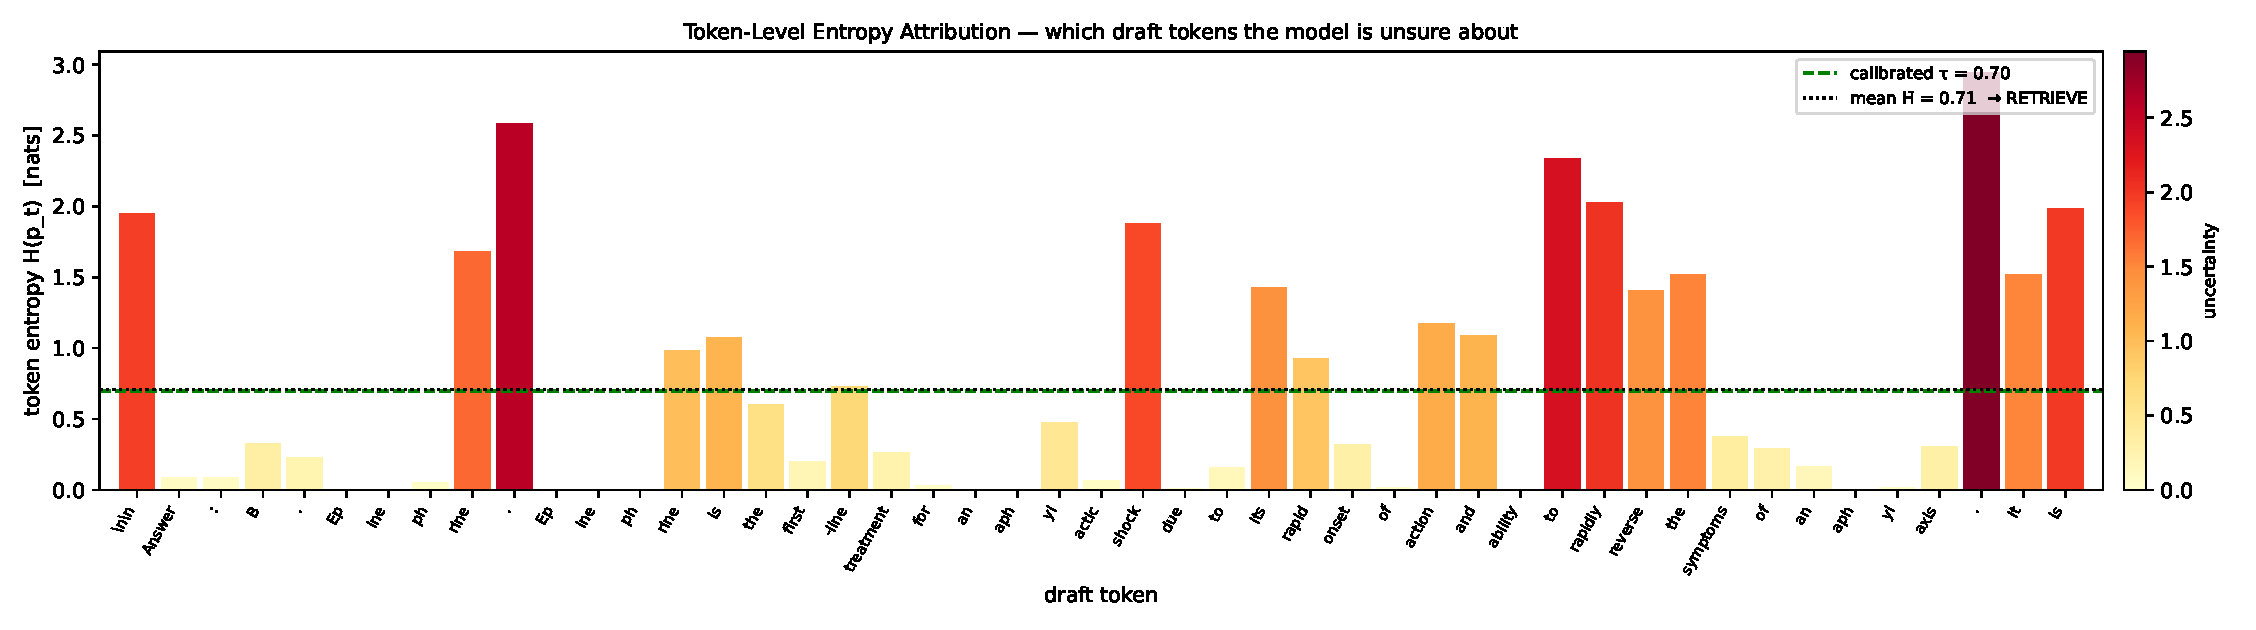
\includegraphics[width=\linewidth]{results/figures/fig_entropy_attribution}
  \caption{Per-token entropy across a drafted answer to \emph{``first-line
    treatment for anaphylaxis''}. High entropy concentrates on filler and
    phrasing tokens; the clinically decisive tokens
    (``Ep/ine/ph/rine'') are generated with near-zero entropy.}
  \label{fig:entropy-attribution}
\end{figure}

Because the entropy gate logs its full per-token array, uncertainty can be
localised rather than merely summarised. Figure~\ref{fig:entropy-attribution}
shows the per-token entropy of a draft answer to a canonical clinical
question. The mean, $\bar{H} = 0.709$, lands almost exactly on the
calibrated threshold $\tau = 0.70$, so the gate marginally votes
\textsc{retrieve} --- a useful demonstration that it discriminates near its
operating point rather than saturating.

The per-token view, however, is the real result, and it is unflattering to
the method: the high-entropy tokens are \emph{filler and phrasing} ---
newlines, punctuation, ``to'', ``is'' --- while the model is near-certain on
the clinically decisive drug-name tokens. Raw token entropy on this model
largely measures \emph{phrasing freedom}, not clinical-content uncertainty.
This is a genuine limitation of entropy gating as implemented, reported as
such: the aggregate signal works well enough to calibrate a useful retrieval
rate, but its per-token composition is not what the method's intuition
promises. It also points directly at the highest-value methodological
successor --- content-token-restricted or attention-weighted entropy
(Section~\ref{sec:conc-future}).

\section{Risk Stratification and the Safety Envelope}
\label{sec:eval-envelope}

% AUTO-GENERATED by scripts/generate_tables.py -- DO NOT EDIT.
% Regenerate with: python scripts/generate_tables.py
% Every number is computed from results/raw_logs/ via evaluation.loading.
% git b3a9d01 | 2026-07-13 13:27
\begin{table}[t]
  \centering
  \begin{tabular}{lccc}
    \toprule
    & \multicolumn{3}{c}{Accuracy \% [95\% Wilson CI]} \\
    \cmidrule(lr){2-4}
    Policy & Low ($n=28$) & Medium ($n=166$) & High ($n=6$) \\
    \midrule
    P1 always-retrieve & 28.6\% [15, 47] & 47.6\% [40, 55] & 66.7\% [30, 90] \\
    P4 hybrid & 28.6\% [15, 47] & 47.6\% [40, 55] & 66.7\% [30, 90] \\
    P3 closed-book$^\dagger$ & 64.3\% [46, 79] & 60.8\% [53, 68] & 83.3\% [44, 97] \\
    P5 gated (calib.) & 50.0\% [33, 67] & 55.4\% [48, 63] & 50.0\% [19, 81] \\
    \bottomrule
  \end{tabular}
  \caption{Multiple-choice accuracy by clinical risk level, with 95\% Wilson score
  intervals. The high-risk stratum contains only $n=6$ questions, giving intervals
  roughly $\pm$30 percentage points wide: \emph{no comparison between policies at high
  risk is statistically meaningful in this evaluation}. The medium stratum
  ($n=166$) is where the headline comparison actually rests, and even there the
  intervals overlap.}
  \label{tab:risk}
\end{table}


\begin{figure}[t]
  \centering
  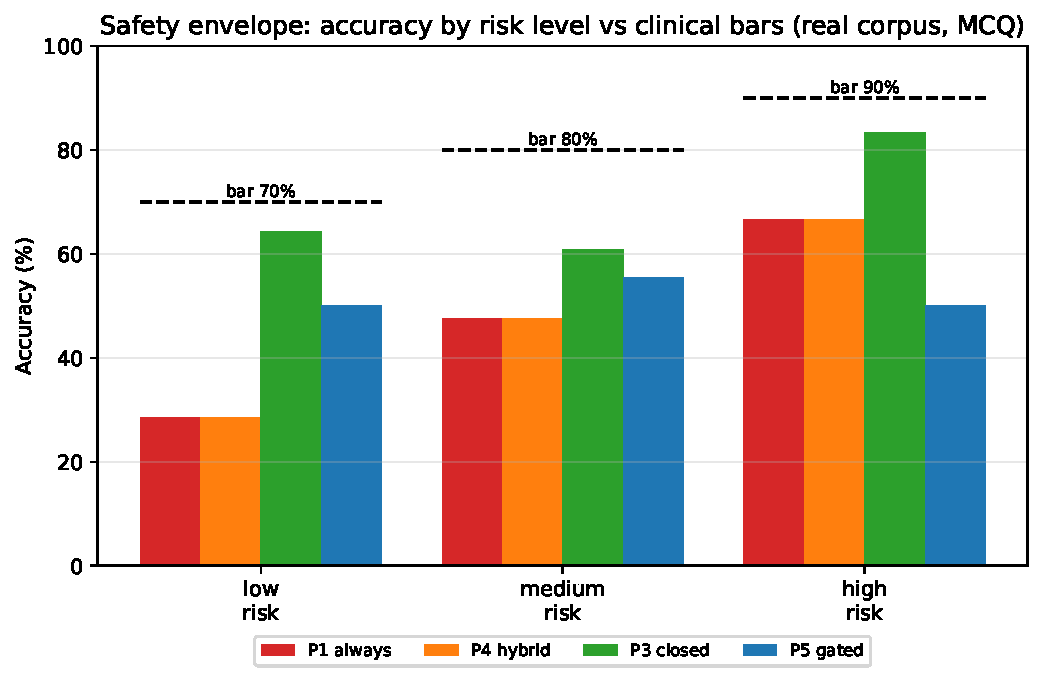
\includegraphics[width=\linewidth]{results/figures/fig_safety_envelope}
  \caption{The safety envelope: policy accuracy by clinical risk level
    against the stipulated bars (\barLow{}/\barMedium{}/\barHigh{}). No
    policy clears any bar.}
  \label{fig:safety-envelope}
\end{figure}

The safety envelope (Section~\ref{sec:method-envelope}) is \textbf{empty}:
no policy clears even the \barLow{} low-risk bar. The best result on the
benchmark, closed-book P3 at \accPthreeMcq{}, falls \gapToLowBar{}pp short.
Two things must be said about this result, and neither is an apology.

First, the emptiness is now attributable to \emph{model capability}, not to
the method or the corpus: retrieval demonstrably works
(Section~\ref{sec:eval-corpus}), the corpus demonstrably contains answers,
and the gate demonstrably routes sensibly --- yet the quantised 3B model
tops out \gapToLowBar{}pp below the lowest bar. The dissertation's honest
output on this axis is a \emph{quantified distance to clinical
acceptability} for a fully offline, CPU-only configuration --- a number that
is useful precisely because nobody should deploy without knowing it.

Second, the statistical honesty. The high-risk stratum contains only
$n=6$ questions; its 95\% Wilson intervals span roughly $\pm 30$pp
(P5 [19\%, 81\%]; P1 [30\%, 90\%]). \textbf{No comparison between policies
at high risk is meaningful at this sample size.} The substantive comparison
rests on the medium stratum ($n=166$), where P5 leads P1 but the intervals
still overlap, and the low stratum ($n=28$), where the gap is widest
(P5 50\% versus P1 29\%).
% [ANALYSIS] evaluation/metrics.py risk_stratified_summary; see tab_risk.

\section{Cost, Latency and the Trade-off Frontier}
\label{sec:eval-cost}

\begin{figure}[t]
  \centering
  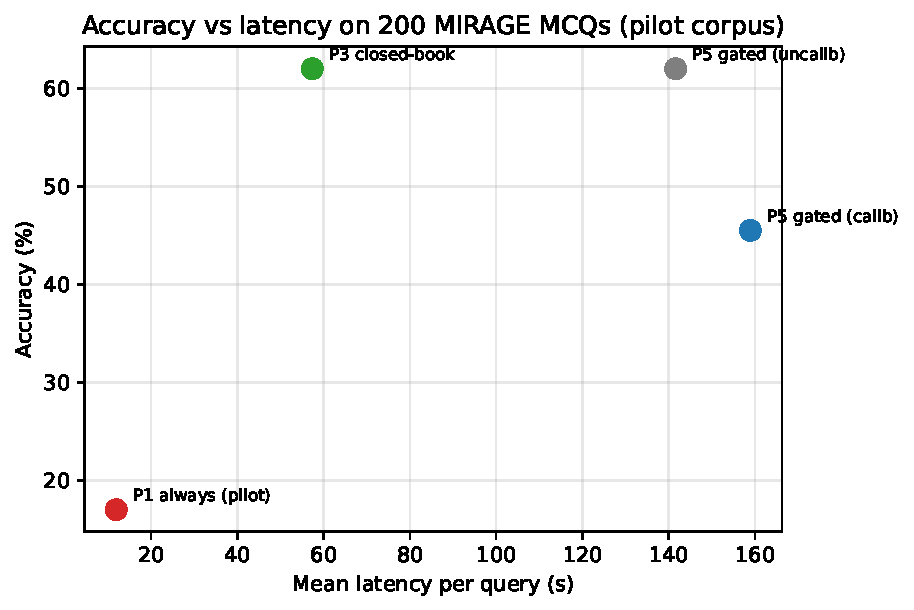
\includegraphics[width=0.8\linewidth]{results/figures/fig_pareto}
  \caption{Accuracy versus mean per-query latency by policy.}
  \label{fig:pareto}
\end{figure}

An uncomfortable engineering truth is stated here rather than hidden behind
the retrieval-rate number: \textbf{P5 is slower in wall-clock terms than
always-retrieve} (\latPfiveMcq{} versus \latPoneMcq{} per query on MCQ). The
ensemble issues three extra draft generations per query --- one shared
entropy/margin draft and two probe drafts --- before the final answer, and
on CPU these drafts dominate. The gate as implemented halves \emph{retrieval
calls} (exactly) but does not save \emph{time} on this hardware.

Whether that trade is worth making depends on what dominates the deployment
cost. On this laptop, generation dominates, so the gate costs time. On a
deployment where retrieval is the expensive resource --- a large corpus on
slow storage, a metered search service, a shared index under load --- halving
retrieval calls is the win the gate delivers. The constructive response is
also concrete: the entropy and margin signals already derive from the
\emph{same} draft, so merging their generations (five model calls per query
to four, an estimated $\sim$20\% latency saving) and evaluating a probe-free
logit-only configuration are the obvious optimisations, quantified as future
work (Section~\ref{sec:conc-future}).

\section{Cross-Model Generalisation}
\label{sec:eval-crossmodel}
% ================= PLACEHOLDER — EXPERIMENT NOT YET RUN =================
% All prerequisites are built and verified (chat-format abstraction proven
% byte-identical for existing logs; Qwen 7B/14B configs; smoke_test_model.py;
% Colab notebook). If the Qwen-7B run (P3+P5, MCQ+open, own calibration)
% completes before submission, report here:
%   - whether calibration non-transfer recurs (expect: different signal
%     range, different tau)
%   - whether selective-beats-always survives at 7B
%   - whether the closed-book ceiling rises toward the safety bars
% If the run does NOT happen, DELETE this section entirely and rely on the
% single-model limitation in §6.2 + future work in §8.2. Do not leave a
% stub section in the submitted PDF.
% ========================================================================

\emph{[Placeholder --- pending Qwen-7B scaling run; see source comment.
Delete this section if the run is not completed before submission.]}
